\subsection{An example: definable subsets of simple graphs with four nodes}

We proceeded to give a complete analysis of the definable subsets of simple graphs with four nodes. First, we classified all the members of $\modn{\sg}{4}$ up to isomorphism. We discovered that any maximal collection of pairwise non-isomorphic graphs in $\modn{\sg}{4}$ has exactly 11 members. We listed such a collection $A_1,\ldots,A_{11}$ and calculated $\card{\orb{A_i}{\symn{4}}}$ and $\card{\aut{A_i}}$ for each $1\leq i\leq 11$. See the tables below. The \emph{complement} $A^c$ of a simple graph $A$ is defined as follows: $U^{A^c}=U^A$; for $a\neq b$, $\op{a}{b}\in L^{A^c}$ if and only if $\op{a}{b}\not\in L^{A}$. In the table of graphs below, each $A_i$ with $i$ odd, is drawn in red, and $A_{i+1} = A_i^c$ is drawn in blue. The exceptional graph $A_{11}$ is drawn in purple since it is isomorphic to its own complement. 

\[
\begin{array}{|c|c|c|c|} 
\hline
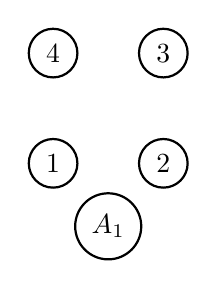
\begin{tikzpicture}
[scale=.2]
\begin{scope}[every node/.style={circle,thick,draw}]
    \node (1) at (0,4) {1};
    \node (2) at (7,4) {2};
    \node (3) at (7,11) {3};
    \node (4) at (0,11) {4};
   \node(A) at (3.5,0) {$A_1$};
\end{scope}

\begin{scope}[%>={Stealth[black]},
              every node/.style={fill=white,circle},
              every edge/.style={draw=red,very thick}]
     %\draw (1) edge  (2);
     %\draw (2) edge  (3);
     %\draw (3) edge  (4);
     %\draw (4) edge  (1);
     %\draw (4) edge  (2);
     %\draw (3) edge  (1);
        
\end{scope}
\end{tikzpicture}
&
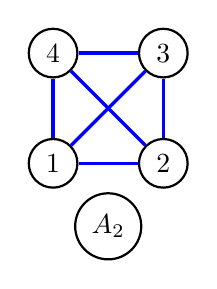
\begin{tikzpicture}
[scale=.2]
\begin{scope}[every node/.style={circle,thick,draw}]
    \node (1) at (0,4) {1};
    \node (2) at (7,4) {2};
    \node (3) at (7,11) {3};
    \node (4) at (0,11) {4};
   \node(A) at (3.5,0) {$A_2$};
\end{scope}

\begin{scope}[%>={Stealth[black]},
              every node/.style={fill=white,circle},
              every edge/.style={draw=blue,very thick}]
     \draw (1) edge  (2);
     \draw (2) edge  (3);
     \draw (3) edge  (4);
     \draw (4) edge  (1);
     \draw (4) edge  (2);
     \draw (3) edge  (1);
             
\end{scope}
\end{tikzpicture}
&
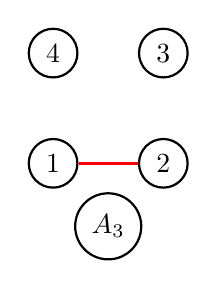
\begin{tikzpicture}
[scale=.2]
\begin{scope}[every node/.style={circle,thick,draw}]
    \node (1) at (0,4) {1};
    \node (2) at (7,4) {2};
    \node (3) at (7,11) {3};
    \node (4) at (0,11) {4};
   \node(A) at (3.5,0) {$A_3$};
\end{scope}

\begin{scope}[%>={Stealth[black]},
              every node/.style={fill=white,circle},
              every edge/.style={draw=red,very thick}]
      \draw (1) edge  (2);
     %\draw (2) edge  (3);
     %\draw (3) edge  (4);
     %\draw (4) edge  (1);
     %\draw (4) edge  (2);
     %\draw (3) edge  (1);             
\end{scope}
\end{tikzpicture}
&
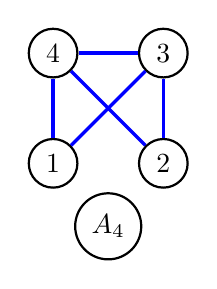
\begin{tikzpicture}
[scale=.2]
\begin{scope}[every node/.style={circle,thick,draw}]
    \node (1) at (0,4) {1};
    \node (2) at (7,4) {2};
    \node (3) at (7,11) {3};
    \node (4) at (0,11) {4};
   \node(A) at (3.5,0) {$A_4$};
\end{scope}

\begin{scope}[%>={Stealth[black]},
              every node/.style={fill=white,circle},
              every edge/.style={draw=blue,very thick}]
     %\draw (1) edge  (2);
     \draw (2) edge  (3);
     \draw (3) edge  (4);
     \draw (4) edge  (1);
     \draw (4) edge  (2);
     \draw (3) edge  (1);
             
\end{scope}
\end{tikzpicture}\\
\hline
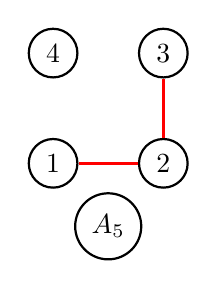
\begin{tikzpicture}
[scale=.2]
\begin{scope}[every node/.style={circle,thick,draw}]
    \node (1) at (0,4) {1};
    \node (2) at (7,4) {2};
    \node (3) at (7,11) {3};
    \node (4) at (0,11) {4};
   \node(A) at (3.5,0) {$A_5$};
\end{scope}

\begin{scope}[%>={Stealth[black]},
              every node/.style={fill=white,circle},
              every edge/.style={draw=red,very thick}]
\draw (1) edge  (2);
     \draw (2) edge  (3);
     %\draw (3) edge  (4);
     %\draw (4) edge  (1);
     %\draw (4) edge  (2);
     %\draw (3) edge  (1);             
\end{scope}
\end{tikzpicture}
&
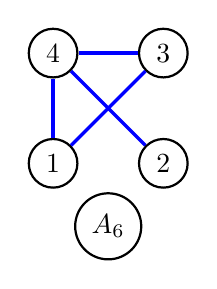
\begin{tikzpicture}
[scale=.2]
\begin{scope}[every node/.style={circle,thick,draw}]
    \node (1) at (0,4) {1};
    \node (2) at (7,4) {2};
    \node (3) at (7,11) {3};
    \node (4) at (0,11) {4};
   \node(A) at (3.5,0) {$A_6$};
\end{scope}

\begin{scope}[%>={Stealth[black]},
              every node/.style={fill=white,circle},
              every edge/.style={draw=blue,very thick}]
%\draw (1) edge  (2);
%     \draw (2) edge  (3);
     \draw (3) edge  (4);
     \draw (4) edge  (1);
     \draw (4) edge  (2);
     \draw (3) edge  (1);
             
\end{scope}
\end{tikzpicture}
&
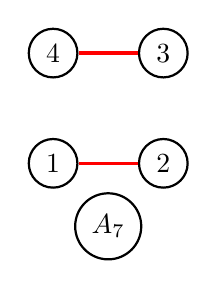
\begin{tikzpicture}
[scale=.2]
\begin{scope}[every node/.style={circle,thick,draw}]
    \node (1) at (0,4) {1};
    \node (2) at (7,4) {2};
    \node (3) at (7,11) {3};
    \node (4) at (0,11) {4};
   \node(A) at (3.5,0) {$A_7$};
\end{scope}

\begin{scope}[%>={Stealth[black]},
              every node/.style={fill=white,circle},
              every edge/.style={draw=red,very thick}]
\draw (1) edge  (2);
     %\draw (2) edge  (3);
     \draw (3) edge  (4);
     %\draw (4) edge  (1);
     %\draw (4) edge  (2);
     %\draw (3) edge  (1);             
\end{scope}
\end{tikzpicture}
&
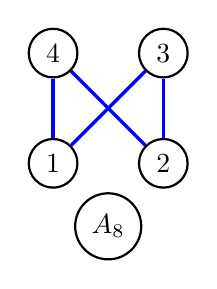
\begin{tikzpicture}
[scale=.2]
\begin{scope}[every node/.style={circle,thick,draw}]
    \node (1) at (0,4) {1};
    \node (2) at (7,4) {2};
    \node (3) at (7,11) {3};
    \node (4) at (0,11) {4};
   \node(A) at (3.5,0) {$A_8$};
\end{scope}

\begin{scope}[%>={Stealth[black]},
              every node/.style={fill=white,circle},
              every edge/.style={draw=blue,very thick}]
%\draw (1) edge  (2);
     \draw (2) edge  (3);
%     \draw (3) edge  (4);
     \draw (4) edge  (1);
     \draw (4) edge  (2);
     \draw (3) edge  (1);
     \end{scope}
\end{tikzpicture}
\\
\hline
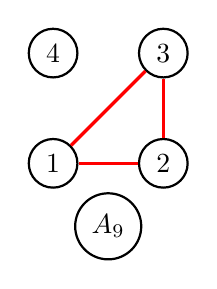
\begin{tikzpicture}
[scale=.2]
\begin{scope}[every node/.style={circle,thick,draw}]
    \node (1) at (0,4) {1};
    \node (2) at (7,4) {2};
    \node (3) at (7,11) {3};
    \node (4) at (0,11) {4};
   \node(A) at (3.5,0) {$A_9$};
\end{scope}

\begin{scope}[%>={Stealth[black]},
              every node/.style={fill=white,circle},
              every edge/.style={draw=red,very thick}]
\draw (1) edge  (2);
     \draw (2) edge  (3);
%     \draw (3) edge  (4);
%     \draw (4) edge  (1);
%     \draw (4) edge  (2);
     \draw (3) edge  (1);
     \end{scope}
\end{tikzpicture}
&
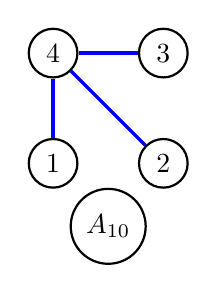
\begin{tikzpicture}
[scale=.2]
\begin{scope}[every node/.style={circle,thick,draw}]
    \node (1) at (0,4) {1};
    \node (2) at (7,4) {2};
    \node (3) at (7,11) {3};
    \node (4) at (0,11) {4};
   \node(A) at (3.5,0) {$A_{10}$};
\end{scope}

\begin{scope}[%>={Stealth[black]},
              every node/.style={fill=white,circle},
              every edge/.style={draw=blue,very thick}]
%\draw (1) edge  (2);
%     \draw (2) edge  (3);
     \draw (3) edge  (4);
     \draw (4) edge  (1);
     \draw (4) edge  (2);
%     \draw (3) edge  (1);
             
\end{scope}
\end{tikzpicture}
&
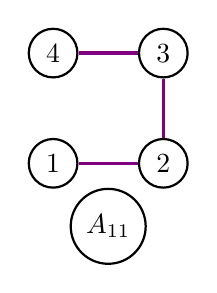
\begin{tikzpicture}
[scale=.2]
\begin{scope}[every node/.style={circle,thick,draw}]
    \node (1) at (0,4) {1};
    \node (2) at (7,4) {2};
    \node (3) at (7,11) {3};
    \node (4) at (0,11) {4};
   \node(A) at (3.5,0) {$A_{11}$};
\end{scope}

\begin{scope}[%>={Stealth[black]},
              every node/.style={fill=white,circle},
              every edge/.style={draw=violet,very thick}]
 \draw (1) edge  (2);
     \draw (2) edge  (3);
     \draw (3) edge  (4);
%     \draw (4) edge  (1);
 %    \draw (4) edge  (2);
  %   \draw (3) edge  (1);
     \end{scope}
\end{tikzpicture}
&
\\
\hline

\end{array}
\]

Note that $\aut{A}=\aut{A^c}$, for every simple graph $A$. This made it quick work to complete the following table.

\[
\begin{array}{|c|c|c|}
\hline
A_i  & \card{\orb{A_i}{\symn{4}}} & \card{\aut{A_i}}\\
\hline
A_1 & 1 & 24\\
\hline
A_2 & 1 & 24 \\
\hline
A_3 & 6 & 4\\
\hline
A_4 & 6 & 4\\
\hline
A_5 & 12 & 2\\
\hline
A_6 & 12 & 2\\
\hline
A_7 & 3 & 8 \\
\hline
A_8 & 3 & 8 \\
\hline
A_9 & 4 & 6 \\
\hline
A_{10} & 4 & 6 \\
\hline
A_{11} & 12 & 2\\
\hline
\end{array}
\]
Note the ``verification'' of the result predicted by the Orbit-Stabilizer Theorem: $\card{\orb{A_i}{\symn{4}}} \cdot \card{\aut{A_i}} = \card{\symn{4}} (= 24)$.
%\subsection{Addendum}

We %began, but did not complete, 
gave a systematic account of which sets are definable in the structures $A_1,\ldots,A_{11}$. The following table, together with Corollary \ref{def-orbs-cor}, suffices. We write $\autorbs{A}$ to denote the collection of orbits of $\aut{A}$ acting on $U^A$. We list only the odd numbered structures, since, as already observed, $\aut{A}=\aut{A^c}$.
\[
\begin{array}{l l}
A_i & \autorbs{A_i}\\
\hline
A_1 & \{[4]\}\\
A_3 & \{\{1,2\},\{3,4\}\}\\
A_5 & \{\{2\},\{4\},\{1,3\}\}\\
A_7 & \{[4]\}\\
A_9 & \{\{1,2,3\},\{4\}\}\\
A_{11} & \{\{1,4\},\{2,3\}\}
\end{array}
\]
\subsection{Additional topics not covered fully in class}
\subsubsection{Automorphisms preserve degree}

Let $A$ be a graph and $a\in U^A$. the \emph{neighborhood of} $a$ in $A$ (written $\nbh{a}{A}$) is $\{b\in U^A\mid\op{a}{b}\in L^A\}$. The \emph{degree of} $a$ in $A$ (written $\dg{a}{A}$) is $\card{\{b\in U^A\mid\op{a}{b}\in L^A\}}$. The next proposition follows directly from the definition of an automorphism.
\begin{proposition}
For every graph $A$, $a\in U^A$, and $h\in\aut{A}$,
\[
h[\nbh{a}{A}]=\nbh{h(a)}{A}.
\]
Hence,
\[
\dg{a}{A} = \dg{h(a)}{A}.
\]
\end{proposition}
\subsubsection{Rigidity}

We introduced the notion of rigidity: a graph $A$ is \emph{rigid} if and only if $\aut{A}=\{e\}$, that is, $A$ has no non-trivial automorphisms. It follows at once from Theorem \ref{fin-aut-def-thm} that if $A$ is a finite rigid structure and $V\subseteq U^A$, then $V\in\Def{A}$.
We noted that no member of $\modn{\sg}{4}$, is rigid, and mused about the question: ``what is the least $n$ such that $\modn{\sg}{n}$ contains a rigid graph?''

\subsubsection{Proof Sketch of Theorem \ref{fin-aut-def-thm}}

We give the argument for graphs; the generalization to structures interpreting multiple polyadic predicates is straightforward.

Suppose $A$ is a finite graph, $a\in U^A$, and $V=\orb{A}{\aut{A}}$. We construct a schema $S(x)$ such that $S[A]=V$. We may suppose without loss of generality that $U^A=[k]$ for some $k\in\mathbb{Z}^+$ and that $a=1$. For each $1\leq i,j\leq k$, let the schema $S_{i,j}$ be $Lx_ix_j$ if $\op{i}{j}\in L^A$, and $\neg Lx_ix_j$ otherwise. Let $S(x)$ be the schema
\[
(\exists x_2)\ldots(\exists x_k)(\bigwedge_{1\leq i,j\leq k}S_{i,j}\wedge\bigwedge_{1\leq i<j\leq k}x_i\neq x_j\wedge(\forall y)\bigvee_{1\leq i\leq k} y=x_i).
\] 
Let $a_1,\dots,a_k$ be a sequence of nodes from $U^A$ and observe that
\[
A\models(\bigwedge_{1\leq i,j\leq k}S_{i,j}\wedge\bigwedge_{1\leq i<j\leq k}x_i\neq x_j\wedge(\forall y)\bigvee_{1\leq i\leq k} y=x_i)[(x_1|a_1),\ldots,(x_k|a_k)]
\]
if and only if the function mapping $i$ to $a_i$ is an automorphism of $A$. \qed
\subsubsection{Proof Sketch of Theorem \ref{aut-thm}}

Theorem \ref{aut-thm} is a corollary of the following more general result concerning isomorphisms of structures.
\begin{theorem}\label{iso-thm}
Suppose $A$ and $B$ are structures and $f$ is an isomorphism of $A$ onto $B$. Then for every schema $S(x_1,\ldots,x_k)$ and sequence of elements $a_1,\dots,a_k\in U^A$,
\begin{equation}\label{iso-eq}
A\models S[(x_1|a_1),\ldots,(x_k|a_k)]\mbox{ iff }B\models S[(x_1|f(a_1)),\ldots,(x_k|f(a_k))].
\end{equation}
\end{theorem}

{\bf Proof sketch of Theorem \ref{iso-thm}}:
We give the argument for graphs; the generalization to structures interpreting multiple polyadic predicates is straightforward.
The argument proceeds by induction on the syntactic structure of schemata. The base case verifies (\ref{iso-eq}) for atomic schemata, that is, schemata of the form $Lx_ix_j$ or $x_i=x_j$, for some $i,j$. In this case, the verification follows directly from the hypothesis that $f$ is an isomorphism from $A$ onto $B$, in particular, that it is edge-preserving and injective.

Suppose $S$ is a truth-functional combination, for example the conjunction, of schemata $S'$ and $S''$, where, as hypothesis of induction, (\ref{iso-eq}) holds for both $S'$ and $S''$. Then,
\[
\begin{array}{lc}
A\models S[(x_1|a_1),\ldots,(x_k|a_k)] & \mbox{ iff}\\
A\models S'[(x_1|a_1),\ldots,(x_k|a_k)]\mbox{ and }A\models S''[(x_1|a_1),\ldots,(x_k|a_k)] & \mbox{ iff}\\
B\models S'[(x_1|f(a_1)),\ldots,(x_k|f(a_k))]\mbox{ and }B\models S''[(x_1|f(a_1)),\ldots,(x_k|f(a_k))] & \mbox{ iff}\\
B\models S[(x_1|f(a_1)),\ldots,(x_k|f(a_k))].
\end{array}
\]
The first and third biconditionals follow from the truth-functional semantics of conjunction, while the second follows from the induction hypothesis.

Finally, suppose that $S$ is $(\exists y)S'(x_1,\ldots,x_k,y)$ and (\ref{iso-eq}) holds for $S'$ (the universal quantifier is handled similarly). Then,
\[
\begin{array}{lc}
A\models S[(x_1|a_1),\ldots,(x_k|a_k)] & \mbox{ iff}\\
\mbox{for some $a\in U^A$ }
A\models S'[(x_1|a_1),\ldots,(x_k|a_k),(y|a)] & \mbox{ iff}\\
\mbox{for some $a\in U^A$ }
B\models S'[(x_1|f(a_1)),\ldots,(x_k|f(a_k)),(y|f(a))] & \mbox{ iff}\\
\mbox{for some $b\in U^B$ }
B\models S'[(x_1|f(a_1)),\ldots,(x_k|f(a_k)),(y|b)] & \mbox{ iff}\\
B\models S[(x_1|f(a_1)),\ldots,(x_k|f(a_k))].
\end{array}
\]
The first and fourth biconditionals follow from the semantics for the existential quantifier, the second from the induction hypothesis, and the third from the hypothesis that $f$ is an isomorphism from $A$ onto $B$, in particular, that it is
surjective. \qed 


